\documentclass[12pt]{article}
\usepackage{amsmath}
\usepackage{amsthm}
\usepackage{amsfonts}
\usepackage{amssymb}
\usepackage{enumerate}
\usepackage{tikz}
\usepackage[margin = .75in]{geometry}
\usepackage{youngtab}
\definecolor{purple}{RGB}{51,0,111} % Official UW color scheme
\usepackage[colorlinks=true, allcolors=purple]{hyperref} %% For links
\pagestyle{empty} %% Gets rid of the page number
%% New Commands 
%% For our common number systems.
\newcommand{\Nn}{\mathbb{N}} 
\newcommand{\Zz}{\mathbb{Z}} 
\newcommand{\Qq}{\mathbb{Q}}
\newcommand{\Rr}{\mathbb{R}}
\newcommand\set[1]{\{ #1 \}} %%\set{abc} ==> {abc}
\newcommand\abs[1]{\left| #1 \right|} %% \abs{abc} ==> |abc|
\newcommand\parens[1]{\left( #1 \right)} 
\newcommand\brac[1]{\left[ #1 \right]} 
\newenvironment{solution}
  {\renewcommand\qedsymbol{$\blacksquare$}\begin{proof}[Solution]}
  {\end{proof}}



\begin{document}
\raggedright
\begin{center}
      {\large Math 1522 Calculus 2 Review: Selected Solutions}\\
  {Fall 2026}\\
\end{center}

\begin{enumerate}
\setcounter{enumi}{0}
\item Formulas to know
\begin{enumerate}
\item[(a)] Derivative and graph of $\sin^{-1}(x)$.
\begin{solution}
$y=\sin^{-1}(x)$ is the inverse of $\sin$ restricted to $[-\frac{\pi}{2},\frac{\pi}{2}]$, so its domain is $[-1,1]$ and its range is $[-\frac{\pi}{2},\frac{\pi}{2}]$. The graph increases from $(-1,-\frac{\pi}{2})$ through $(0,0)$ to $(1,\frac{\pi}{2})$, with vertical tangents at the ends.
\[ \frac{d}{dx}\sin^{-1}(x)=\frac{1}{\sqrt{1-x^2}}, \qquad -1<x<1. \]
\end{solution}

\item[(h)] State the Inverse Function Theorem.
\begin{solution}
Let $f$ be a 1-1 differentiable function with inverse $f^{-1}$, and let $a$ be in the domain of $f^{-1}$. If $f'(f^{-1}(a))\neq 0$, then $f^{-1}$ is differentiable at $a$ and
\[ (f^{-1})'(a)=\frac{1}{f'(f^{-1}(a))}. \]
The tangent line to $f$ at $(b,a)$, where $b=f^{-1}(a)$, reflected across $y=x$ is the tangent line to $f^{-1}$ at $(a,b)$, and reflecting swaps rise and run.
\end{solution}

\end{enumerate}

\setcounter{enumi}{1}
\item Logarithmic differentiation
\begin{enumerate}
\item[(a)] Find $y'$ if $y=x^{\sqrt{x}}$.
\begin{solution}
Take $\ln$ of both sides: $\ln y=\sqrt{x}\,\ln x$. Differentiate implicitly.
\[ \frac{y'}{y}=\frac{\ln x}{2\sqrt{x}}+\frac{\sqrt{x}}{x}, \qquad y'=x^{\sqrt{x}}\left(\frac{\ln x}{2\sqrt{x}}+\frac{1}{\sqrt{x}}\right)=x^{\sqrt{x}}\,\frac{\ln x+2}{2\sqrt{x}}. \]
\end{solution}

\item[(c)] Find $y'$ if $y=(\sin x)^{\sin x}$.
\begin{solution}
$\ln y=\sin x\,\ln(\sin x)$, so
\[ \frac{y'}{y}=\cos x\,\ln(\sin x)+\sin x\cdot\frac{\cos x}{\sin x}=\cos x\,\bigl(\ln(\sin x)+1\bigr), \]
\[ y'=(\sin x)^{\sin x}\cos x\,\bigl(\ln(\sin x)+1\bigr). \]
\end{solution}

\item[(d)] Find $y'(0)$ if $y=\frac{(x+1)^4e^x}{\sqrt{1+3x}}$.
\begin{solution}
Take $\ln$ of both sides and expand: $\ln y=4\ln(x+1)+x-\frac12\ln(1+3x)$. Differentiate implicitly.
\[ \frac{y'}{y}=\frac{4}{x+1}+1-\frac{3}{2(1+3x)}. \]
At $x=0$, $y=1$, so $y'(0)=4+1-\frac32=\frac72$.
\end{solution}

\end{enumerate}

\setcounter{enumi}{2}
\item Derivatives of logarithms
\begin{enumerate}
\item[(c)] Find $y$ if $y'=\frac{\sin(x)}{\cos(x)}$.
\begin{solution}
Let $u=\cos x$, so $du=-\sin x\,dx$.
\[ y=\int\frac{\sin x}{\cos x}\,dx=-\int\frac{du}{u}=-\ln|\cos x|+C=\ln|\sec x|+C. \]
\end{solution}

\item[(d)] Find the domain and range of $f(x)=\ln(\sqrt{9-e^x})$.
\begin{solution}
We need $9-e^x>0$, that is $x<\ln 9$. So the domain is $(-\infty,\ln 9)$. On this domain $e^x$ takes every value in $(0,9)$, so $\sqrt{9-e^x}$ takes every value in $(0,3)$, and $\ln$ of that takes every value in $(-\infty,\ln 3)$. The range is $(-\infty,\ln 3)$.
\end{solution}

\item[(f)] Let $f(x)=3-e^{-x}$. Find the domain and range of $f$, find $f^{-1}(x)$, and state the domain and range of $f^{-1}$. Does the graph of $f$ have a horizontal asymptote?
\begin{solution}
$f$ is defined for every $x$, so the domain is $(-\infty,\infty)$. The values of $e^{-x}$ fill $(0,\infty)$, so the range of $f$ is $(-\infty,3)$.

Inverse: set $y=3-e^{-x}$ and solve for $x$. Then $e^{-x}=3-y$, so $x=-\ln(3-y)$. Swapping names,
\[ f^{-1}(x)=-\ln(3-x), \]
with domain $(-\infty,3)$ (the range of $f$) and range $(-\infty,\infty)$ (the domain of $f$).

As $x\to\infty$, $e^{-x}\to0$ so $f(x)\to3$. The line $y=3$ is a horizontal asymptote.
\end{solution}

\item[(g)] Find $y'(1)$ if $y=3^x\log_3(x)$.
\begin{solution}
Product rule, with $\frac{d}{dx}3^x=3^x\ln 3$ and $\frac{d}{dx}\log_3 x=\frac{1}{x\ln 3}$.
\[ y'=3^x\ln 3\,\log_3(x)+\frac{3^x}{x\ln 3}, \qquad y'(1)=3\ln3\cdot 0+\frac{3}{\ln 3}=\frac{3}{\ln 3}. \]
\end{solution}

\end{enumerate}

\setcounter{enumi}{3}
\item Inverse trig functions
\begin{enumerate}
\item[(a)] Prove the identity $\frac{d}{dx}\sec^{-1}(x)=\frac{1}{x\sqrt{x^2-1}}$ (ignore domain issues).
\begin{solution}
Let $y=\sec^{-1}(x)$, so $\sec y=x$. Differentiate implicitly: $\sec y\tan y\;y'=1$. From $\tan^2y=\sec^2y-1=x^2-1$ we get $\tan y=\sqrt{x^2-1}$ (taking $y$ in $[0,\frac{\pi}{2})$, where $\tan y\ge0$). So
\[ y'=\frac{1}{\sec y\tan y}=\frac{1}{x\sqrt{x^2-1}}. \]
\end{solution}

\item[(d)] Find $y$ if $y'=\frac{x^2}{\frac19+x^6}$.
\begin{solution}
Let $u=x^3$, so $du=3x^2\,dx$.
\[ y=\frac13\int\frac{du}{\frac19+u^2}=\frac13\cdot 9\int\frac{du}{1+(3u)^2}=\frac13\cdot 9\cdot\frac13\tan^{-1}(3u)+C=\tan^{-1}(3x^3)+C. \]
\end{solution}

\item[(f)] Find the equation of the tangent line to $y=2\tan^{-1}(x^2)$ at $x=1$.
\begin{solution}
The point is $y(1)=2\tan^{-1}(1)=\frac{\pi}{2}$. The slope is
\[ y'=2\cdot\frac{2x}{1+x^4}, \qquad y'(1)=2. \]
So the tangent line is $y=\frac{\pi}{2}+2(x-1)$.
\end{solution}

\item[(g)] Write $\cos(\tan^{-1}(x/2))$ as an algebraic function of $x$.
\begin{solution}
Let $\theta=\tan^{-1}(x/2)$, so $\tan\theta=\frac{x}{2}$ with $-\frac{\pi}{2}<\theta<\frac{\pi}{2}$. Draw a right triangle with opposite side $x$ and adjacent side $2$. The hypotenuse is $\sqrt{4+x^2}$, and $\cos\theta>0$ on this range, so
\[ \cos(\tan^{-1}(x/2))=\frac{2}{\sqrt{4+x^2}}. \]
\end{solution}

\item[(h)] Find $y$ if $y'=\frac{x}{\sqrt{1-x^4}}$.
\begin{solution}
Let $u=x^2$, so $du=2x\,dx$.
\[ y=\frac12\int\frac{du}{\sqrt{1-u^2}}=\frac12\sin^{-1}(x^2)+C. \]
\end{solution}

\end{enumerate}

\setcounter{enumi}{4}
\item Hyperbolic functions
\begin{enumerate}
\item[(b)] Find $\cosh^{-1}(2)$.
\begin{solution}
Solve $\cosh y=2$, that is $\frac{e^y+e^{-y}}{2}=2$. Multiply by $2e^y$: $e^{2y}-4e^y+1=0$, a quadratic in $e^y$. So $e^y=2\pm\sqrt3$ and $y=\ln(2\pm\sqrt3)$. Since $(2-\sqrt3)(2+\sqrt3)=1$, the two solutions are $y=\pm\ln(2+\sqrt3)$. The function $\cosh^{-1}$ is the inverse of $\cosh$ restricted to $[0,\infty)$, so
\[ \cosh^{-1}(2)=\ln(2+\sqrt3). \]
\end{solution}

\item[(d)] Evaluate $\lim_{x\to\infty}\coth x$.
\begin{solution}
Divide the top and bottom by $e^x$.
\[ \lim_{x\to\infty}\coth x=\lim_{x\to\infty}\frac{e^x+e^{-x}}{e^x-e^{-x}}=\lim_{x\to\infty}\frac{1+e^{-2x}}{1-e^{-2x}}=\frac{1+0}{1-0}=1. \]
\end{solution}

\item[(f)] Prove that the derivative of $\tanh x$ is $\operatorname{sech}^2x$.
\begin{solution}
Write $\tanh x=\frac{\sinh x}{\cosh x}$ and use the quotient rule with $(\sinh x)'=\cosh x$, $(\cosh x)'=\sinh x$.
\[ \frac{d}{dx}\tanh x=\frac{\cosh x\cosh x-\sinh x\sinh x}{\cosh^2x}=\frac{1}{\cosh^2x}=\operatorname{sech}^2x, \]
using $\cosh^2x-\sinh^2x=1$.
\end{solution}

\item[(g)] Find $y'$ if $y=\tan^{-1}(\sinh x)$, and simplify.
\begin{solution}
\[ y'=\frac{\cosh x}{1+\sinh^2x}=\frac{\cosh x}{\cosh^2x}=\frac{1}{\cosh x}=\operatorname{sech}x. \]
\end{solution}

\item[(h)] Evaluate $\int_{-\ln3}^{\ln3}\cosh x\,dx$.
\begin{solution}
\[ \int_{-\ln3}^{\ln3}\cosh x\,dx=\sinh(\ln3)-\sinh(-\ln3)=2\sinh(\ln 3)=e^{\ln3}-e^{-\ln3}=3-\frac13=\frac83. \]
\end{solution}

\end{enumerate}

\setcounter{enumi}{5}
\item Inverse Function Theorem
\begin{enumerate}
\item[(a)] Show $f(x)=x+x^3+2x^5$ is 1-1, then find the derivative of $f^{-1}$ at $(4,f^{-1}(4))$.
\begin{solution}
$f'(x)=1+3x^2+10x^4\ge1>0$, so $f$ is increasing, hence 1-1. Since $f(1)=1+1+2=4$, we have $f^{-1}(4)=1$, and
\[ (f^{-1})'(4)=\frac{1}{f'(1)}=\frac{1}{14}. \]
\end{solution}

\item[(b)] $f(x)=5x+2\sin x+2\cos x$, at $(2,f^{-1}(2))$.
\begin{solution}
$f'(x)=5+2\cos x-2\sin x$. Since $|2\cos x-2\sin x|\le 2\sqrt2<5$, $f'(x)>0$ and $f$ is 1-1. Since $f(0)=2$, $f^{-1}(2)=0$, and
\[ (f^{-1})'(2)=\frac{1}{f'(0)}=\frac{1}{5+2}=\frac17. \]
\end{solution}

\item[(i)] Let $f(x)=x+e^x$. Find the equation of the tangent line to the graph of $f^{-1}$ at $x=1$.
\begin{solution}
$f(0)=0+1=1$, so $f^{-1}(1)=0$ and the point is $(1,0)$. $f'(x)=1+e^x$, so $(f^{-1})'(1)=\frac{1}{f'(0)}=\frac12$. The tangent line is
\[ y=\tfrac12(x-1). \]
\end{solution}

\item[(j)] Let $f(x)=2x^3+\ln x+\sin(\pi x)$ for $x>0$ (assume $f$ is 1-1). Find the slope of the tangent line to the graph of $f^{-1}$ at $x=2$.
\begin{solution}
$f(1)=2+0+0=2$, so $f^{-1}(2)=1$. $f'(x)=6x^2+\frac1x+\pi\cos(\pi x)$, so $f'(1)=6+1-\pi$. The slope is
\[ (f^{-1})'(2)=\frac{1}{f'(1)}=\frac{1}{7-\pi}. \]
\end{solution}

\end{enumerate}

\setcounter{enumi}{6}
\item L'H\^opital's rule
\begin{enumerate}
\item[(c)] $\lim_{x\to0^+}x^x$
\begin{solution}
This is the form $0^0$. Let $y=x^x$, so $\ln y=x\ln x=\dfrac{\ln x}{1/x}$, the form $\frac{-\infty}{\infty}$.
\[ \lim_{x\to0^+}\frac{\ln x}{1/x}\overset{H}{=}\lim_{x\to0^+}\frac{1/x}{-1/x^2}=\lim_{x\to0^+}(-x)=0. \]
So $\ln y\to0$ and $x^x\to e^0=1$.
\end{solution}

\item[(g)] $\lim_{x\to0^+}(1+\sin(2x))^{\cot x}$
\begin{solution}
The form $1^\infty$. Let $y$ be the expression, so $\ln y=\cot x\,\ln(1+\sin 2x)=\dfrac{\ln(1+\sin2x)}{\tan x}$, the form $\frac00$.
\[ \lim_{x\to0^+}\frac{\ln(1+\sin2x)}{\tan x}\overset{H}{=}\lim_{x\to0^+}\frac{\frac{2\cos 2x}{1+\sin2x}}{\sec^2x}=\frac{2}{1}=2. \]
So the limit is $e^2$.
\end{solution}

\item[(i)] $\lim_{x\to0^+}\left(\frac1x-\frac{1}{e^x-1}\right)$
\begin{solution}
The form $\infty-\infty$. Combine into one fraction, then apply L'Hopital twice (each step is $\frac00$).
\[ \lim_{x\to0^+}\frac{e^x-1-x}{x(e^x-1)}\overset{H}{=}\lim_{x\to0^+}\frac{e^x-1}{e^x-1+xe^x}\overset{H}{=}\lim_{x\to0^+}\frac{e^x}{2e^x+xe^x}=\frac12. \]
\end{solution}

\item[(j)] $\lim_{x\to1^-}\frac{\ln x}{\cos^{-1}(x)}$
\begin{solution}
The form $\frac00$, since $\ln1=0$ and $\cos^{-1}(1)=0$.
\[ \lim_{x\to1^-}\frac{\ln x}{\cos^{-1}(x)}\overset{H}{=}\lim_{x\to1^-}\frac{1/x}{-1/\sqrt{1-x^2}}=\lim_{x\to1^-}\left(-\frac{\sqrt{1-x^2}}{x}\right)=0. \]
\end{solution}

\item[(k)] $\lim_{x\to\infty}x\left(\frac{\pi}{2}-\tan^{-1}(2x)\right)$
\begin{solution}
The form $\infty\cdot0$, since $\tan^{-1}(2x)\to\frac{\pi}{2}$. Rewrite as a quotient of the form $\frac00$.
\[ \lim_{x\to\infty}\frac{\frac{\pi}{2}-\tan^{-1}(2x)}{1/x}\overset{H}{=}\lim_{x\to\infty}\frac{-\frac{2}{1+4x^2}}{-\frac{1}{x^2}}=\lim_{x\to\infty}\frac{2x^2}{1+4x^2}=\frac12. \]
\end{solution}

\item[(l)] $\lim_{x\to\infty}\sin^{-1}\left(\frac{e^x}{2e^x+1}\right)$
\begin{solution}
No L'Hopital needed. Divide by $e^x$ inside: $\dfrac{e^x}{2e^x+1}=\dfrac{1}{2+e^{-x}}\to\dfrac12$. Since $\sin^{-1}$ is continuous at $\frac12$,
\[ \lim_{x\to\infty}\sin^{-1}\left(\frac{e^x}{2e^x+1}\right)=\sin^{-1}\left(\tfrac12\right)=\frac{\pi}{6}. \]
\end{solution}

\item[(m)] $\lim_{x\to\infty}\frac{\cosh(\ln x)}{x}$
\begin{solution}
Use the definition: $\cosh(\ln x)=\frac{e^{\ln x}+e^{-\ln x}}{2}=\frac{x+\frac1x}{2}$. So
\[ \lim_{x\to\infty}\frac{\cosh(\ln x)}{x}=\lim_{x\to\infty}\frac{1+\frac{1}{x^2}}{2}=\frac12. \]
\end{solution}

\end{enumerate}

\setcounter{enumi}{7}
\item Substitution
\begin{enumerate}
\item[(a)] $\int_0^{(\pi/2)^{1/3}}x^2\sin x^3\,dx$
\begin{solution}
Let $u=x^3$, $du=3x^2\,dx$. The bounds become $u=0$ and $u=\frac{\pi}{2}$.
\[ \frac13\int_0^{\pi/2}\sin u\,du=\frac13\Bigl[-\cos u\Bigr]_0^{\pi/2}=\frac13(0+1)=\frac13. \]
\end{solution}

\item[(d)] $\int_{\pi/4}^{\pi/2}\cot x\,dx$
\begin{solution}
Let $u=\sin x$, $du=\cos x\,dx$. The bounds become $u=\frac{\sqrt2}{2}$ and $u=1$.
\[ \int_{\sqrt2/2}^{1}\frac{du}{u}=\ln1-\ln\frac{\sqrt2}{2}=\ln\sqrt2=\frac{\ln 2}{2}. \]
\end{solution}

\item[(e)] $\int_1^e\frac{(\ln x)^2}{x}\,dx$
\begin{solution}
Let $u=\ln x$, $du=\frac{dx}{x}$. The bounds become $u=0$ and $u=1$.
\[ \int_0^1u^2\,du=\frac13. \]
\end{solution}

\item[(f)] $\int\frac{\cos x}{4+\sin^2x}\,dx$
\begin{solution}
Let $u=\sin x$, $du=\cos x\,dx$.
\[ \int\frac{du}{4+u^2}=\frac12\tan^{-1}\left(\frac u2\right)+C=\frac12\tan^{-1}\left(\frac{\sin x}{2}\right)+C. \]
\end{solution}

\item[(g)] $\int\frac{dx}{\sqrt x\,(1+\sqrt x)}$
\begin{solution}
Let $u=1+\sqrt x$, $du=\frac{dx}{2\sqrt x}$.
\[ \int\frac{2\,du}{u}=2\ln|u|+C=2\ln(1+\sqrt x)+C. \]
\end{solution}

\end{enumerate}

\setcounter{enumi}{8}
\item Integration by parts
\begin{enumerate}
\item[(b)] $\int_1^e x^4\ln(x)\,dx$
\begin{solution}
Let $u=\ln x$, $dv=x^4\,dx$, so $du=\frac{dx}{x}$, $v=\frac{x^5}{5}$.
\[ \int x^4\ln x\,dx=\frac{x^5\ln x}{5}-\int\frac{x^4}{5}\,dx=\frac{x^5\ln x}{5}-\frac{x^5}{25}+C. \]
\[ \int_1^e x^4\ln x\,dx=\left(\frac{e^5}{5}-\frac{e^5}{25}\right)-\left(0-\frac1{25}\right)=\frac{4e^5+1}{25}. \]
\end{solution}

\item[(e)] $\int_0^\pi e^x\sin(x)\,dx$
\begin{solution}
Call the antiderivative $I=\int e^x\sin x\,dx$. Parts with $u=\sin x$, $dv=e^x\,dx$, then again with $u=\cos x$, $dv=e^x\,dx$:
\[ I=e^x\sin x-\int e^x\cos x\,dx=e^x\sin x-e^x\cos x-I. \]
So $I=\frac{e^x(\sin x-\cos x)}{2}+C$, and
\[ \int_0^\pi e^x\sin x\,dx=\frac{e^\pi(0+1)}{2}-\frac{1\cdot(0-1)}{2}=\frac{e^\pi+1}{2}. \]
\end{solution}

\item[(g)] $\int x\sec^2(x)\,dx$
\begin{solution}
Let $u=x$, $dv=\sec^2x\,dx$, so $du=dx$, $v=\tan x$.
\[ \int x\sec^2x\,dx=x\tan x-\int\tan x\,dx=x\tan x+\ln|\cos x|+C. \]
\end{solution}

\item[(h)] $\int x\sin(2x)\,dx$
\begin{solution}
Let $u=x$, $dv=\sin2x\,dx$, so $du=dx$, $v=-\frac{\cos2x}{2}$.
\[ \int x\sin2x\,dx=-\frac{x\cos2x}{2}+\int\frac{\cos2x}{2}\,dx=-\frac{x\cos2x}{2}+\frac{\sin2x}{4}+C. \]
\end{solution}

\item[(i)] $\int_0^1x\tan^{-1}(x)\,dx$
\begin{solution}
Let $u=\tan^{-1}x$, $dv=x\,dx$, so $du=\frac{dx}{1+x^2}$, $v=\frac{x^2}{2}$.
\[ \int x\tan^{-1}x\,dx=\frac{x^2}{2}\tan^{-1}x-\frac12\int\frac{x^2}{1+x^2}\,dx=\frac{x^2}{2}\tan^{-1}x-\frac12\bigl(x-\tan^{-1}x\bigr)+C, \]
using $\frac{x^2}{1+x^2}=1-\frac{1}{1+x^2}$. At the bounds,
\[ \int_0^1x\tan^{-1}x\,dx=\frac{\pi}{8}-\frac12\left(1-\frac{\pi}{4}\right)=\frac{\pi}{4}-\frac12. \]
\end{solution}

\end{enumerate}

\setcounter{enumi}{9}
\item Trig integrals
\begin{enumerate}
\item[(a)] $\int\sin^3(x)\cos^2(x)\,dx$
\begin{solution}
The power of $\sin$ is odd, so save one $\sin x$ and convert the rest with $\sin^2x=1-\cos^2x$. Let $u=\cos x$, $du=-\sin x\,dx$.
\[ \int(1-\cos^2x)\cos^2x\sin x\,dx=-\int(u^2-u^4)\,du=-\frac{\cos^3x}{3}+\frac{\cos^5x}{5}+C. \]
\end{solution}

\item[(f)] $\int\tan^2(x)\,dx$
\begin{solution}
Use $\tan^2x=\sec^2x-1$.
\[ \int(\sec^2x-1)\,dx=\tan x-x+C. \]
\end{solution}

\item[(h)] $\int\tan^2(x)\sec^4(x)\,dx$
\begin{solution}
The power of $\sec$ is even, so save $\sec^2x$ and convert the other $\sec^2x=1+\tan^2x$. Let $u=\tan x$, $du=\sec^2x\,dx$.
\[ \int\tan^2x(1+\tan^2x)\sec^2x\,dx=\int(u^2+u^4)\,du=\frac{\tan^3x}{3}+\frac{\tan^5x}{5}+C. \]
\end{solution}

\item[(i)] $\int\sin(3x)\cos(2x)\,dx$
\begin{solution}
Use the product formula $\sin A\cos B=\frac12[\sin(A+B)+\sin(A-B)]$ with $A=3x$, $B=2x$.
\[ \frac12\int(\sin5x+\sin x)\,dx=-\frac{\cos5x}{10}-\frac{\cos x}{2}+C. \]
\end{solution}

\item[(j)] $\int_0^{\pi/3}\tan(x)\sec^3(x)\,dx$
\begin{solution}
Save $\sec x\tan x$ and let $u=\sec x$, $du=\sec x\tan x\,dx$. The bounds become $u=1$ and $u=2$.
\[ \int_0^{\pi/3}\sec^2x\,(\sec x\tan x)\,dx=\int_1^2u^2\,du=\frac{8-1}{3}=\frac73. \]
\end{solution}

\end{enumerate}

\setcounter{enumi}{10}
\item Trig substitution
\begin{enumerate}
\item[(a)] $\int_2^3\frac{dx}{(x^2-1)^{3/2}}$
\begin{solution}
Let $x=\sec\theta$, $dx=\sec\theta\tan\theta\,d\theta$, so $(x^2-1)^{3/2}=\tan^3\theta$ (for $0\le\theta<\frac{\pi}{2}$).
\[ \int\frac{\sec\theta\tan\theta}{\tan^3\theta}\,d\theta=\int\frac{\cos\theta}{\sin^2\theta}\,d\theta=-\frac{1}{\sin\theta}+C=-\frac{x}{\sqrt{x^2-1}}+C, \]
since $\sin\theta=\frac{\sqrt{x^2-1}}{x}$ from the triangle with hypotenuse $x$ and adjacent side $1$.
\[ \int_2^3\frac{dx}{(x^2-1)^{3/2}}=-\frac{3}{\sqrt8}+\frac{2}{\sqrt3}=\frac{2\sqrt3}{3}-\frac{3\sqrt2}{4}. \]
\end{solution}

\item[(g)] $\int\frac{dx}{(6-8x-x^2)^{3/2}}$
\begin{solution}
Complete the square: $6-8x-x^2=22-(x+4)^2$. Let $x+4=\sqrt{22}\sin\theta$, $dx=\sqrt{22}\cos\theta\,d\theta$, so $22-(x+4)^2=22\cos^2\theta$.
\[ \int\frac{\sqrt{22}\cos\theta}{22^{3/2}\cos^3\theta}\,d\theta=\frac1{22}\int\sec^2\theta\,d\theta=\frac{\tan\theta}{22}+C=\frac{x+4}{22\sqrt{6-8x-x^2}}+C. \]
\end{solution}

\item[(h)] $\int_0^{\sqrt3}\frac{x^3}{\sqrt{x^2+1}}\,dx$
\begin{solution}
Let $x=\tan\theta$, $dx=\sec^2\theta\,d\theta$, so $\sqrt{x^2+1}=\sec\theta$. The bounds become $\theta=0$ and $\theta=\frac{\pi}{3}$.
\[ \int_0^{\pi/3}\tan^3\theta\sec\theta\,d\theta=\int_0^{\pi/3}(\sec^2\theta-1)\sec\theta\tan\theta\,d\theta. \]
Let $w=\sec\theta$, $dw=\sec\theta\tan\theta\,d\theta$, with bounds $w=1$ and $w=2$.
\[ \int_1^2(w^2-1)\,dw=\left[\frac{w^3}{3}-w\right]_1^2=\frac23+\frac23=\frac43. \]
\end{solution}

\item[(i)] $\int_{\sqrt2}^2\frac{dx}{x^2\sqrt{x^2-1}}$
\begin{solution}
Let $x=\sec\theta$, $dx=\sec\theta\tan\theta\,d\theta$, so $\sqrt{x^2-1}=\tan\theta$. The bounds become $\theta=\frac{\pi}{4}$ and $\theta=\frac{\pi}{3}$.
\[ \int_{\pi/4}^{\pi/3}\frac{\sec\theta\tan\theta}{\sec^2\theta\tan\theta}\,d\theta=\int_{\pi/4}^{\pi/3}\cos\theta\,d\theta=\frac{\sqrt3}{2}-\frac{\sqrt2}{2}. \]
\end{solution}

\item[(j)] $\int_0^1\frac{dx}{(1+x^2)^2}$
\begin{solution}
Let $x=\tan\theta$, $dx=\sec^2\theta\,d\theta$, so $(1+x^2)^2=\sec^4\theta$. The bounds become $\theta=0$ and $\theta=\frac{\pi}{4}$.
\[ \int_0^{\pi/4}\cos^2\theta\,d\theta=\left[\frac\theta2+\frac{\sin2\theta}{4}\right]_0^{\pi/4}=\frac{\pi}{8}+\frac14. \]
\end{solution}

\end{enumerate}

\setcounter{enumi}{11}
\item Partial fractions
\begin{enumerate}
\item[(a)(ii)] $\int\frac{3x^2+6x+2}{x^2+3x+2}\,dx$
\begin{solution}
The degrees are equal, so divide first: $\frac{3x^2+6x+2}{x^2+3x+2}=3-\frac{3x+4}{(x+1)(x+2)}$. Write $\frac{3x+4}{(x+1)(x+2)}=\frac{A}{x+1}+\frac{B}{x+2}$, so $3x+4=A(x+2)+B(x+1)$. At $x=-1$, $A=1$. At $x=-2$, $B=2$.
\[ \int\left(3-\frac{1}{x+1}-\frac{2}{x+2}\right)dx=3x-\ln|x+1|-2\ln|x+2|+C. \]
\end{solution}

\item[(b)(iv)] $\int\frac{x+4}{x^3-4x}\,dx$
\begin{solution}
Factor $x^3-4x=x(x-2)(x+2)$ and write $\frac{x+4}{x(x-2)(x+2)}=\frac Ax+\frac{B}{x-2}+\frac{D}{x+2}$ (we use $D$ to keep $C$ for the constant). Then $x+4=A(x-2)(x+2)+Bx(x+2)+Dx(x-2)$. At $x=0$, $4=-4A$, so $A=-1$. At $x=2$, $6=8B$, so $B=\frac34$. At $x=-2$, $2=8D$, so $D=\frac14$.
\[ \int\frac{x+4}{x^3-4x}\,dx=-\ln|x|+\frac34\ln|x-2|+\frac14\ln|x+2|+C. \]
\end{solution}

\item[(c)(ii)] $\int\frac{3x^2-x+8}{x^3+4x}\,dx$
\begin{solution}
$x^3+4x=x(x^2+4)$ with $x^2+4$ irreducible. Write $\frac{3x^2-x+8}{x(x^2+4)}=\frac Ax+\frac{Bx+D}{x^2+4}$, so $3x^2-x+8=A(x^2+4)+(Bx+D)x$. At $x=0$, $A=2$. Matching $x^2$: $3=A+B$, so $B=1$. Matching $x$: $D=-1$.
\[ \int\left(\frac2x+\frac{x}{x^2+4}-\frac{1}{x^2+4}\right)dx=2\ln|x|+\frac12\ln(x^2+4)-\frac12\tan^{-1}\left(\frac x2\right)+C. \]
\end{solution}

\item[(c)(iii)] Set up, but do not solve, the partial fraction decomposition of $\frac{x+1}{x^2(x-3)(x^2+1)^2}$.
\begin{solution}
Each power of a linear factor gets a constant on top, and each power of an irreducible quadratic gets a linear term on top.
\[ \frac{x+1}{x^2(x-3)(x^2+1)^2}=\frac Ax+\frac{B}{x^2}+\frac{D}{x-3}+\frac{Ex+F}{x^2+1}+\frac{Gx+H}{(x^2+1)^2}. \]
\end{solution}

\end{enumerate}

\setcounter{enumi}{12}
\item Improper integrals
\begin{enumerate}
\item[(b)] $\int_0^1\frac{\ln x}{x}\,dx$
\begin{solution}
The integrand is undefined at $0$. With $u=\ln x$, an antiderivative is $\frac{(\ln x)^2}{2}$.
\[ \lim_{t\to0^+}\int_t^1\frac{\ln x}{x}\,dx=\lim_{t\to0^+}\left(0-\frac{(\ln t)^2}{2}\right)=-\infty. \]
It diverges. The region between the graph and the $x$-axis over $(0,1]$, below the axis and running down along the $y$-axis, has infinite area.
\end{solution}

\item[(f)] $\int_1^\infty\frac{dx}{x^p}$ (consider $p\le1$ and $p>1$)
\begin{solution}
If $p=1$: $\lim_{t\to\infty}\ln t=\infty$, divergent. If $p\neq1$:
\[ \lim_{t\to\infty}\int_1^t x^{-p}\,dx=\lim_{t\to\infty}\frac{t^{1-p}-1}{1-p}. \]
For $p>1$ the exponent $1-p$ is negative, so $t^{1-p}\to0$ and the integral is $\frac{1}{p-1}$. For $p<1$, $t^{1-p}\to\infty$ and it diverges. So it converges exactly when $p>1$.
\end{solution}

\item[(l)] $\int_0^\infty e^{x^2}\,dx$ (don't determine the value)
\begin{solution}
For $x\ge0$, $x^2\ge0$, so $e^{x^2}\ge1$. Then
\[ \int_0^te^{x^2}\,dx\ge\int_0^t1\,dx=t\to\infty, \]
so the integral diverges to $\infty$ by comparison. The region under the graph over $[0,\infty)$ contains a strip of height $1$ and infinite length, so it has infinite area.
\end{solution}

\item[(n)] $\int_0^\infty\frac{e^x}{(1+e^x)^3}\,dx$
\begin{solution}
Let $u=1+e^x$, $du=e^x\,dx$; $x=0$ gives $u=2$ and $x\to\infty$ gives $u\to\infty$.
\[ \lim_{t\to\infty}\int_2^{t}u^{-3}\,du=\lim_{t\to\infty}\left(\frac{1}{2\cdot 4}-\frac{1}{2t^2}\right)=\frac18. \]
\end{solution}

\item[(o)] $\int_1^\infty\frac{\ln x}{x^3}\,dx$
\begin{solution}
Parts with $u=\ln x$, $dv=x^{-3}\,dx$, so $du=\frac{dx}{x}$, $v=-\frac{1}{2x^2}$.
\[ \int\frac{\ln x}{x^3}\,dx=-\frac{\ln x}{2x^2}+\int\frac{dx}{2x^3}=-\frac{\ln x}{2x^2}-\frac{1}{4x^2}+C. \]
\[ \lim_{t\to\infty}\left(-\frac{\ln t}{2t^2}-\frac{1}{4t^2}+\frac14\right)=\frac14, \]
since $\frac{\ln t}{t^2}\to0$ by L'Hopital.
\end{solution}

\item[(p)] $\int_0^2\frac{dx}{(x-1)^{2/3}}$
\begin{solution}
The integrand blows up at $x=1$, inside the interval, so split there. An antiderivative is $3(x-1)^{1/3}$.
\[ \lim_{t\to1^-}\Bigl[3(x-1)^{1/3}\Bigr]_0^t+\lim_{s\to1^+}\Bigl[3(x-1)^{1/3}\Bigr]_s^2=(0+3)+(3-0)=6. \]
Both pieces converge, so the integral converges to $6$.
\end{solution}

\item[(q)] $\int_2^\infty\frac{dx}{4+x^2}$
\begin{solution}
\[ \lim_{t\to\infty}\left[\frac12\tan^{-1}\left(\frac x2\right)\right]_2^t=\frac12\cdot\frac{\pi}{2}-\frac12\cdot\frac{\pi}{4}=\frac{\pi}{8}. \]
\end{solution}

\end{enumerate}

\setcounter{enumi}{13}
\item Numerical integration
\begin{enumerate}
\item[(c)] $\int_0^1(x^3-3x^2+2x+1)\,dx$: over or under estimates, then $M_4$ and $T_4$.
\begin{solution}
Let $f(x)=x^3-3x^2+2x+1$. Then $f''(x)=6x-6<0$ on $[0,1)$, so $f$ is concave down. A concave down graph lies below its chords and above its tangent lines, so the trapezoid rule underestimates and the midpoint rule overestimates. $f'(x)=3x^2-6x+2$ changes sign at $x=1-\frac{1}{\sqrt3}$, so $f$ is not monotonic on $[0,1]$, and the left and right endpoint rules are not determined by this reasoning.

With $\Delta x=\frac14$, $M_4=\frac14\bigl(f(\tfrac18)+f(\tfrac38)+f(\tfrac58)+f(\tfrac78)\bigr)=\frac{161}{128}\approx1.258$ and $T_4=\frac18\bigl(f(0)+2f(\tfrac14)+2f(\tfrac12)+2f(\tfrac34)+f(1)\bigr)=\frac{79}{64}\approx1.234$. The exact value is $\frac14-1+1+1=\frac54$, between them as predicted.
\end{solution}

\item[(d)] Use the trapezoid rule with $n=3$ to approximate $\int_0^32^x\,dx$ in exact form.
\begin{solution}
$\Delta x=1$ and the nodes are $0,1,2,3$.
\[ T_3=\frac12\bigl(2^0+2\cdot2^1+2\cdot2^2+2^3\bigr)=\frac12(1+4+8+8)=\frac{21}{2}. \]
(The exact value is $\frac{7}{\ln2}\approx10.10$. $2^x$ is concave up, so $T_3$ overestimates.)
\end{solution}

\item[(e)] How large must $n$ be so that the trapezoid rule approximates $\int_1^2\frac{dx}{x}$ with error less than $10^{-4}$?
\begin{solution}
$f(x)=\frac1x$ has $f''(x)=\frac{2}{x^3}$, which on $[1,2]$ is at most $2$. So take $K=2$, $b-a=1$.
\[ |E_T|\le\frac{2}{12n^2}=\frac{1}{6n^2}<10^{-4}\iff n^2>\frac{10^4}{6}\approx1666.7. \]
So $n\ge41$ is enough.
\end{solution}

\end{enumerate}

\setcounter{enumi}{14}
\item Sequences
\begin{enumerate}
\item[(e)] If an alternating sequence converges, what must it converge to?
\begin{solution}
It must converge to $0$. Suppose $a_n\to L$ and the terms alternate in sign. The positive terms are a subsequence converging to $L$, so $L\ge0$. The negative terms also converge to $L$, so $L\le0$. Hence $L=0$.
\end{solution}

\item[(h)] Write $\{-\frac18,\frac1{27},-\frac1{64},\frac1{125},\dots\}$ as a function of $n$.
\begin{solution}
The denominators are $2^3,3^3,4^3,5^3$ and the signs alternate starting negative. So $a_n=\dfrac{(-1)^n}{(n+1)^3}$ for $n\ge1$.
\end{solution}

\item[(j)] Monotonic? Bounded? $a_n=1+\frac{(-1)^n}{n}$ and $b_n=\frac{n}{n+1}$ ($n\ge1$).
\begin{solution}
$a_1=0$, $a_2=\frac32$, $a_3=\frac23$, $a_4=\frac54$: it goes up, down, up, so $a_n$ is not monotonic. Since $\left|\frac{(-1)^n}{n}\right|\le1$, $0\le a_n\le2$, so it is bounded.

$b_n=1-\frac{1}{n+1}$, and $\frac{1}{n+1}$ decreases, so $b_n$ is increasing. It is bounded: $\frac12\le b_n<1$.
\end{solution}

\item[(k)] Show that $\lim_{n\to\infty}\frac{3^n}{n!}=0$.
\begin{solution}
For $n\ge3$, write the quotient as a product of $n$ factors and bound the middle ones by $1$:
\[ 0<\frac{3^n}{n!}=\frac31\cdot\frac32\cdot\frac33\cdot\frac34\cdots\frac{3}{n-1}\cdot\frac3n\le\frac31\cdot\frac32\cdot\frac3n=\frac{27}{2n}. \]
Since $\frac{27}{2n}\to0$, the Squeeze Theorem gives $\frac{3^n}{n!}\to0$.
\end{solution}

\end{enumerate}

\setcounter{enumi}{15}
\item Test for Divergence (TFD)
\begin{enumerate}
\item[(a)] $\sum_{n=1}^\infty\frac{(-1)^nn}{n+1}$
\begin{solution}
$\left|\frac{(-1)^nn}{n+1}\right|=\frac{n}{n+1}\to1$, so the terms do not go to $0$ (they approach $1$ and $-1$ alternately). By the TFD the series diverges.
\end{solution}

\item[(c)] $\sum_{n=0}^\infty\frac{n^2+1}{6n^2+6n+1}$
\begin{solution}
$\lim_{n\to\infty}\frac{n^2+1}{6n^2+6n+1}=\frac16\neq0$, so the series diverges by the TFD.
\end{solution}

\item[(e)] Can you use the TFD on $\sum_{n=2}^\infty\frac{1}{n^2}$?
\begin{solution}
No. The TFD only concludes divergence when $a_n\not\to0$. Here $\frac1{n^2}\to0$, so the TFD says nothing. (The series converges, as a $p$-series with $p=2$.)
\end{solution}

\item[(f)] $\sum_{n=1}^\infty2^{1/n}$
\begin{solution}
$2^{1/n}\to2^0=1\neq0$, so the series diverges by the TFD.
\end{solution}

\item[(g)] Suppose $b_n>0$ and $\sum b_n$ converges. What does the TFD say about $\sum\frac{1}{b_n}$?
\begin{solution}
Since $\sum b_n$ converges, $b_n\to0$. As $b_n>0$, this means $\frac1{b_n}\to\infty$, so the terms of $\sum\frac1{b_n}$ do not go to $0$. By the TFD, $\sum\frac1{b_n}$ diverges.
\end{solution}

\end{enumerate}

\setcounter{enumi}{16}
\item Telescoping series
\begin{enumerate}
\item[(a)] $\sum_{n=2}^\infty\frac{1}{n^2-1}$
\begin{solution}
Partial fractions: $\frac{1}{n^2-1}=\frac12\left(\frac{1}{n-1}-\frac{1}{n+1}\right)$. In the partial sum $s_N=\sum_{n=2}^N$, everything cancels except the first two positive terms and the last two negative ones.
\[ s_N=\frac12\left(1+\frac12-\frac1N-\frac1{N+1}\right)\to\frac12\cdot\frac32=\frac34. \]
\end{solution}

\item[(c)] $\sum_{n=1}^\infty\left[\tan^{-1}(n+2)-\tan^{-1}(n)\right]$
\begin{solution}
Each term cancels against the term two places later.
\[ s_N=\tan^{-1}(N+1)+\tan^{-1}(N+2)-\tan^{-1}(1)-\tan^{-1}(2). \]
As $N\to\infty$, $s_N\to\frac{\pi}{2}+\frac{\pi}{2}-\frac{\pi}{4}-\tan^{-1}(2)=\frac{3\pi}{4}-\tan^{-1}(2)$.
\end{solution}

\item[(d)] $\sum_{n=1}^\infty\left[f(n)-f(n+1)\right]$, where $\lim_{n\to\infty}f(n)=L$
\begin{solution}
$s_N=\bigl(f(1)-f(2)\bigr)+\bigl(f(2)-f(3)\bigr)+\cdots+\bigl(f(N)-f(N+1)\bigr)=f(1)-f(N+1)$. So the sum is $f(1)-L$.
\end{solution}

\item[(e)] $\sum_{n=1}^\infty\left[f(n)-f(n+k)\right]$, $k$ a positive integer, $\lim f(n)=L$
\begin{solution}
For $N\ge k$, every $f(m)$ with $k<m\le N$ appears once with each sign, so
\[ s_N=\bigl(f(1)+\cdots+f(k)\bigr)-\bigl(f(N+1)+\cdots+f(N+k)\bigr)\to f(1)+\cdots+f(k)-kL. \]
\end{solution}

\item[(f)] Determine if $\sum_{n=1}^\infty\ln\left(1+\frac1n\right)$ converges or diverges by writing out its partial sums.
\begin{solution}
$\ln\left(1+\frac1n\right)=\ln\frac{n+1}{n}=\ln(n+1)-\ln n$, so the partial sums telescope.
\[ s_N=(\ln2-\ln1)+(\ln3-\ln2)+\cdots+\bigl(\ln(N+1)-\ln N\bigr)=\ln(N+1)\to\infty. \]
The series diverges. (The TFD says nothing here, since the terms do go to $0$.)
\end{solution}

\end{enumerate}

\setcounter{enumi}{17}
\item Geometric series
\begin{enumerate}
\item[(b)] $\sum_{n=0}^\infty\frac{4^{2n-1}}{17^n}$
\begin{solution}
$\frac{4^{2n-1}}{17^n}=\frac14\left(\frac{16}{17}\right)^n$, geometric with first term $\frac14$ and ratio $r=\frac{16}{17}$, $|r|<1$.
\[ \sum_{n=0}^\infty\frac14\left(\frac{16}{17}\right)^n=\frac{1/4}{1-16/17}=\frac{17}{4}. \]
\end{solution}

\item[(c)] $\sum_{n=-4}^\infty\left(\frac12\right)^n$
\begin{solution}
The first term is $\left(\frac12\right)^{-4}=16$ and $r=\frac12$. So the sum is $\frac{16}{1-1/2}=32$.
\end{solution}

\item[(d)] $\sum_{n=1}^\infty\frac{3^{n+1}}{4^{n-1}}$
\begin{solution}
The first term ($n=1$) is $\frac{9}{1}=9$ and the ratio is $r=\frac34$.
\[ \sum_{n=1}^\infty\frac{3^{n+1}}{4^{n-1}}=\frac{9}{1-3/4}=36. \]
\end{solution}

\item[(e)] $2-1+\frac12-\frac14+\frac18-\cdots$
\begin{solution}
Geometric with first term $2$ and $r=-\frac12$. The sum is $\frac{2}{1+1/2}=\frac43$.
\end{solution}

\item[(f)] For which $a$ does $\sum_{k=1}^\infty\left(\frac{2a}{1+a^2}\right)^k$ converge? Find its value.
\begin{solution}
Let $r=\frac{2a}{1+a^2}$. The series converges exactly when $|r|<1$. Since $(|a|-1)^2\ge0$, we get $2|a|\le1+a^2$, so $|r|\le1$, with equality exactly when $|a|=1$. So the series converges for all $a\neq\pm1$. Its first term is $r$, so
\[ \sum_{k=1}^\infty r^k=\frac{r}{1-r}=\frac{2a}{1+a^2-2a}=\frac{2a}{(a-1)^2}. \]
\end{solution}

\end{enumerate}

\setcounter{enumi}{18}
\item Integral Test
\begin{enumerate}
\item[(a)] $\sum_{n=2}^\infty\frac{1}{n(\ln n)^2}$
\begin{solution}
$f(x)=\frac{1}{x(\ln x)^2}$ is positive, continuous, and decreasing on $[2,\infty)$. With $u=\ln x$,
\[ \int_2^\infty\frac{dx}{x(\ln x)^2}=\lim_{t\to\infty}\left(\frac{1}{\ln2}-\frac{1}{\ln t}\right)=\frac{1}{\ln2}. \]
The integral converges, so the series converges.
\end{solution}

\item[(c)] Show $\sum_{n=1}^\infty\frac{1}{n^p}$ converges if $p>1$ and diverges if $0<p\le1$.
\begin{solution}
For $p>0$, $f(x)=x^{-p}$ is positive, continuous, and decreasing on $[1,\infty)$. By problem 13(f), $\int_1^\infty x^{-p}\,dx$ converges exactly when $p>1$. By the Integral Test the series converges for $p>1$ and diverges for $0<p\le1$, including $p=1$, where $\int_1^\infty\frac{dx}{x}=\lim_{t\to\infty}\ln t=\infty$.
\end{solution}

\item[(d)] $\sum_{n=1}^\infty ne^{-n^2}$
\begin{solution}
$f(x)=xe^{-x^2}$ is positive and continuous, and $f'(x)=e^{-x^2}(1-2x^2)<0$ for $x\ge1$, so it is decreasing on $[1,\infty)$. With $u=x^2$,
\[ \int_1^\infty xe^{-x^2}\,dx=\lim_{t\to\infty}\frac{e^{-1}-e^{-t^2}}{2}=\frac{1}{2e}. \]
The integral converges, so the series converges.
\end{solution}

\item[(e)] Can you use the integral test on $\sum_{n=1}^\infty\frac{2+\sin n}{n^2}$?
\begin{solution}
No. The Integral Test needs $f(x)=\frac{2+\sin x}{x^2}$ to be decreasing, and it is not: the numerator oscillates, so $f$ increases on stretches where $\sin x$ rises quickly. Use the DCT instead: $0<\frac{2+\sin n}{n^2}\le\frac{3}{n^2}$, and $\sum\frac{3}{n^2}$ converges ($p=2$). So the series converges.
\end{solution}

\end{enumerate}

\setcounter{enumi}{19}
\item p-series
\begin{enumerate}
\item[(a)] $\sum_{n=5}^\infty\frac{1}{n^e}$
\begin{solution}
A $p$-series with $p=e>1$ (starting at $n=5$ does not change convergence). It converges.
\end{solution}

\item[(c)] $\sum_{n=1}^\infty\frac{1}{n^{0.000001}}$
\begin{solution}
A $p$-series with $p=10^{-6}\le1$. It diverges, no matter how slowly.
\end{solution}

\item[(d)] $\sum_{n=1}^\infty\frac{n^2+\sqrt n}{n^4}$
\begin{solution}
Split the term: $\frac{n^2+\sqrt n}{n^4}=\frac{1}{n^2}+\frac{1}{n^{7/2}}$. Both are $p$-series with $p>1$ ($p=2$ and $p=\frac72$), and a sum of two convergent series converges. So the series converges.
\end{solution}

\item[(e)] For which $p$ does $\sum_{n=1}^\infty\frac{1}{n^{2p-1}}$ converge?
\begin{solution}
It is a $p$-series with exponent $2p-1$, so it converges exactly when $2p-1>1$, that is $p>1$.
\end{solution}

\end{enumerate}

\setcounter{enumi}{20}
\item Direct Comparison Test (DCT) and Limit Comparison Test (LCT)
\begin{enumerate}
\item[(b)] $\sum_{n=1}^\infty\sin(1/n)$
\begin{solution}
The terms are positive. Compare with $b_n=\frac1n$, using $\lim_{x\to0}\frac{\sin x}{x}=1$:
\[ \lim_{n\to\infty}\frac{\sin(1/n)}{1/n}=1. \]
The limit is positive and finite and $\sum\frac1n$ diverges, so by the LCT the series diverges.
\end{solution}

\item[(c)] $\sum_{n=0}^\infty\frac{\tan^{-1}(n)}{n^2+1}$
\begin{solution}
$0\le\tan^{-1}(n)<\frac{\pi}{2}$, so for $n\ge1$, $0\le\frac{\tan^{-1}n}{n^2+1}\le\frac{\pi/2}{n^2}$. Since $\sum\frac{\pi/2}{n^2}$ converges ($p=2$), the DCT shows the series converges. (The $n=0$ term is $0$ and does not matter.)
\end{solution}

\item[(f)] $\sum_{n=1}^\infty\frac{1}{2^n+n}$
\begin{solution}
$0<\frac{1}{2^n+n}<\frac{1}{2^n}$, and $\sum\left(\frac12\right)^n$ is a convergent geometric series ($|r|=\frac12<1$). By the DCT the series converges.
\end{solution}

\item[(g)] $\sum_{n=1}^\infty\frac{n^2-2n}{n^{7/2}+1}$
\begin{solution}
The terms are positive for $n\ge3$, and the first two terms do not affect convergence. For large $n$ the term behaves like $\frac{n^2}{n^{7/2}}=\frac{1}{n^{3/2}}$, so compare with $b_n=\frac{1}{n^{3/2}}$.
\[ \lim_{n\to\infty}\frac{(n^2-2n)\,n^{3/2}}{n^{7/2}+1}=\lim_{n\to\infty}\frac{1-\frac2n}{1+n^{-7/2}}=1. \]
Since $\sum\frac{1}{n^{3/2}}$ converges, the LCT shows the series converges.
\end{solution}

\item[(h)] $\sum_{n=1}^\infty\frac{1}{n^2+n\cos n}$
\begin{solution}
$n^2+n\cos n\ge n^2-n\ge0$, with $1+\cos1>0$ at $n=1$, so the terms are positive. Compare with $b_n=\frac1{n^2}$:
\[ \lim_{n\to\infty}\frac{n^2}{n^2+n\cos n}=\lim_{n\to\infty}\frac{1}{1+\frac{\cos n}{n}}=1, \]
since $\left|\frac{\cos n}{n}\right|\le\frac1n\to0$. By the LCT the series converges.
\end{solution}

\end{enumerate}

\setcounter{enumi}{21}
\item Alternating Series Test (AST)
\begin{enumerate}
\item[(a)] $\sum_{n=2}^\infty\frac{(-1)^n}{n\ln n}$
\begin{solution}
Let $b_n=\frac{1}{n\ln n}$. For $n\ge2$, $b_n>0$, and $n\ln n$ is increasing to $\infty$, so $b_n$ is decreasing and $b_n\to0$. By the AST it converges.
\end{solution}

\item[(b)] $\sum_{i=1}^\infty\frac{\cos(\pi i)}{i^{0.1}}$
\begin{solution}
$\cos(\pi i)=(-1)^i$, so this is $\sum(-1)^ib_i$ with $b_i=\frac{1}{i^{0.1}}$. Then $b_i>0$, $b_i$ is decreasing, and $b_i\to0$. By the AST it converges.
\end{solution}

\item[(c)] $\sum_{k=2}^\infty\frac{(-1)^{k+15}}{\ln k}$
\begin{solution}
$(-1)^{k+15}=-(-1)^k$, so this is $-\sum(-1)^kb_k$ with $b_k=\frac1{\ln k}$. Since $\ln k$ increases to $\infty$, $b_k$ is positive, decreasing, and $b_k\to0$. By the AST it converges.
\end{solution}

\item[(d)] $\sum_{n=1}^\infty\frac{(-1)^n\ln n}{\sqrt n}$
\begin{solution}
Let $b_n=\frac{\ln n}{\sqrt n}$ and $f(x)=\frac{\ln x}{\sqrt x}$. Then $f'(x)=\frac{2-\ln x}{2x^{3/2}}<0$ for $x>e^2\approx7.4$, so $b_n$ is decreasing for $n\ge8$. By L'Hopital, $\lim_{x\to\infty}\frac{\ln x}{\sqrt x}=\lim_{x\to\infty}\frac{1/x}{1/(2\sqrt x)}=\lim_{x\to\infty}\frac{2}{\sqrt x}=0$. The AST applies from $n=8$ on, and the first seven terms do not affect convergence. It converges.
\end{solution}

\item[(e)] $\sum_{n=1}^\infty\frac{(-1)^n\sqrt n}{n+4}$
\begin{solution}
Let $b_n=\frac{\sqrt n}{n+4}$ and $f(x)=\frac{\sqrt x}{x+4}$. Then
\[ f'(x)=\frac{\frac{x+4}{2\sqrt x}-\sqrt x}{(x+4)^2}=\frac{4-x}{2\sqrt x\,(x+4)^2}<0 \quad\text{for } x>4, \]
so $b_n$ is decreasing for $n\ge4$. Dividing top and bottom by $\sqrt n$, $b_n=\frac{1}{\sqrt n+4/\sqrt n}\to0$. The AST applies from $n=4$ on, so the series converges.
\end{solution}

\item[(f)] $a_n=\frac1n$ for $n$ odd, $a_n=\frac1{n^2}$ for $n$ even. Can you use the AST on $\sum(-1)^na_n$?
\begin{solution}
No. The AST needs $a_n$ decreasing, but $a_2=\frac14<a_3=\frac13$, and this happens at every even $n$. (The series actually diverges. Its even terms form the convergent series $\sum\frac{1}{(2m)^2}$, and its odd terms form $-\sum\frac{1}{2m-1}$, which diverges. A convergent series plus a divergent one diverges.)
\end{solution}

\end{enumerate}

\setcounter{enumi}{22}
\item Ratio Test
\begin{enumerate}
\item[(b)] $\sum_{n=0}^\infty\frac{n!}{n^n}$
\begin{solution}
(Start at $n=1$, since $0^0$ is undefined.) With $a_n=\frac{n!}{n^n}$,
\[ \frac{a_{n+1}}{a_n}=\frac{(n+1)!}{(n+1)^{n+1}}\cdot\frac{n^n}{n!}=\left(\frac{n}{n+1}\right)^n=\frac{1}{\left(1+\frac1n\right)^n}\to\frac1e<1. \]
By the Ratio Test it converges.
\end{solution}

\item[(c)] $\sum_{n=0}^\infty\frac{(2n+1)!}{3^n}$
\begin{solution}
\[ \frac{a_{n+1}}{a_n}=\frac{(2n+3)!}{3^{n+1}}\cdot\frac{3^n}{(2n+1)!}=\frac{(2n+3)(2n+2)}{3}\to\infty. \]
By the Ratio Test it diverges.
\end{solution}

\item[(d)] $\sum_{n=1}^\infty\frac{n^24^n}{n!}$
\begin{solution}
\[ \frac{a_{n+1}}{a_n}=\frac{(n+1)^24^{n+1}}{(n+1)!}\cdot\frac{n!}{n^24^n}=\frac{4(n+1)}{n^2}\to0<1. \]
By the Ratio Test it converges.
\end{solution}

\end{enumerate}

\setcounter{enumi}{23}
\item Root Test
\begin{enumerate}
\item[(a)] $\sum_{n=1}^\infty\left(\frac{2n+1}{3n-1}\right)^n$
\begin{solution}
\[ \sqrt[n]{a_n}=\frac{2n+1}{3n-1}\to\frac23<1. \]
By the Root Test it converges.
\end{solution}

\item[(b)] $\sum_{n=1}^\infty\frac{n^n}{2^{n^2}}$
\begin{solution}
\[ \sqrt[n]{a_n}=\frac{n}{2^n}\to0<1 \]
(by L'Hopital, $\lim_{x\to\infty}\frac{x}{2^x}=\lim_{x\to\infty}\frac{1}{2^x\ln2}=0$). By the Root Test it converges.
\end{solution}

\item[(c)] Show the Root Test is inconclusive for $\sum\frac1n$ and $\sum\frac1{n^2}$. Which converges?
\begin{solution}
First, $\ln\bigl(n^{1/n}\bigr)=\frac{\ln n}{n}\to0$, so $n^{1/n}\to1$. Then
\[ \sqrt[n]{\tfrac1n}=\frac{1}{n^{1/n}}\to1, \qquad \sqrt[n]{\tfrac1{n^2}}=\frac{1}{\left(n^{1/n}\right)^2}\to1. \]
Both limits equal $1$, where the Root Test says nothing. Yet $\sum\frac1{n^2}$ converges ($p=2$) and $\sum\frac1n$ diverges ($p=1$).
\end{solution}

\item[(d)] $\sum_{n=1}^\infty\frac{2^n}{n^5}$: Root Test? Ratio Test?
\begin{solution}
Both work. Root: $\sqrt[n]{a_n}=\frac{2}{\left(n^{1/n}\right)^5}\to2>1$. Ratio: $\frac{a_{n+1}}{a_n}=2\left(\frac{n}{n+1}\right)^5\to2>1$. Either way the series diverges.
\end{solution}

\end{enumerate}

\setcounter{enumi}{24}
\item Absolute and conditional convergence
\begin{enumerate}
\item[(a)] $\sum_{n=1}^\infty\frac{(-1)^n}{n}$
\begin{solution}
$\sum\left|\frac{(-1)^n}{n}\right|=\sum\frac1n$ diverges, so it is not absolutely convergent. With $b_n=\frac1n$ positive, decreasing, and $b_n\to0$, the AST shows it converges. So it converges conditionally.
\end{solution}

\item[(c)] $\sum_{k=1}^\infty\frac{k\cos(\pi k)}{k^3+1}$
\begin{solution}
$\cos(\pi k)=(-1)^k$, so $|a_k|=\frac{k}{k^3+1}$. Compare with $\frac1{k^2}$:
\[ \lim_{k\to\infty}\frac{k\cdot k^2}{k^3+1}=1. \]
Since $\sum\frac1{k^2}$ converges, $\sum|a_k|$ converges by the LCT. The series converges absolutely.
\end{solution}

\item[(d)] $\sum_{n=1}^\infty\frac{(-1)^nn^3}{2^n}$
\begin{solution}
Apply the Ratio Test to $|a_n|=\frac{n^3}{2^n}$:
\[ \frac{|a_{n+1}|}{|a_n|}=\frac12\left(\frac{n+1}{n}\right)^3\to\frac12<1. \]
So $\sum|a_n|$ converges, and the series converges absolutely.
\end{solution}

\item[(e)] $\sum_{n=1}^\infty\frac{(-1)^nn}{n^2+1}$
\begin{solution}
Absolute values: $\frac{n}{n^2+1}$ compared with $\frac1n$ gives $\lim\frac{n^2}{n^2+1}=1$, so $\sum\frac{n}{n^2+1}$ diverges by the LCT. AST: $b_n=\frac{n}{n^2+1}\to0$, and $f(x)=\frac{x}{x^2+1}$ has $f'(x)=\frac{1-x^2}{(x^2+1)^2}\le0$ for $x\ge1$, so $b_n$ is decreasing. The series converges conditionally.
\end{solution}

\item[(f)] Suppose $\sum a_n$ converges to $2$. What is $\lim a_n$? Must $\sum|a_n|$ converge?
\begin{solution}
Since the series converges, $\lim_{n\to\infty}a_n=0$. No, $\sum|a_n|$ need not converge. The series $\sum_{n=1}^\infty\frac{(-1)^{n+1}}{n}$ converges to $\ln2$ but not absolutely. Multiplying every term by $\frac{2}{\ln2}$ gives a series that converges to $2$ whose absolute values still form a multiple of the harmonic series.
\end{solution}

\end{enumerate}

\setcounter{enumi}{25}
\item Radius of Convergence (ROC) and Interval of Convergence (IOC)
\begin{enumerate}
\item[(a)] $\sum_{n=0}^\infty n^nx^n$
\begin{solution}
For $x\neq0$, the Ratio Test gives
\[ \left|\frac{(n+1)^{n+1}x^{n+1}}{n^nx^n}\right|=(n+1)\left(1+\frac1n\right)^n|x|\to\infty. \]
So the series diverges for every $x\neq0$. ROC $R=0$, IOC $\{0\}$.
\end{solution}

\item[(e)] $\sum_{n=1}^\infty\frac{(-1)^nx^{2n}}{3^n(2n+1)}$
\begin{solution}
Ratio Test:
\[ \left|\frac{a_{n+1}}{a_n}\right|=\frac{x^2}{3}\cdot\frac{2n+1}{2n+3}\to\frac{x^2}{3}. \]
It converges when $x^2<3$, so $R=\sqrt3$. At $x=\pm\sqrt3$, $x^{2n}=3^n$ and the series is $\sum\frac{(-1)^n}{2n+1}$, which converges by the AST. IOC $[-\sqrt3,\sqrt3]$.
\end{solution}

\item[(f)] $\sum_{n=1}^\infty\frac{(x+2)^n}{n\,4^n}$
\begin{solution}
Ratio Test: $\left|\frac{a_{n+1}}{a_n}\right|=\frac{|x+2|}{4}\cdot\frac{n}{n+1}\to\frac{|x+2|}{4}$. So it converges for $|x+2|<4$: center $-2$, $R=4$. At $x=2$: $\sum\frac1n$ diverges. At $x=-6$: $\sum\frac{(-1)^n}{n}$ converges by the AST. IOC $[-6,2)$.
\end{solution}

\item[(g)] Center, ROC, IOC: $\sum_{n=1}^\infty\frac{2^n(x-3)^n}{n^2}$
\begin{solution}
The center is $3$. Ratio Test: $\left|\frac{a_{n+1}}{a_n}\right|=2|x-3|\left(\frac{n}{n+1}\right)^2\to2|x-3|$, so $R=\frac12$. At $x=\frac72$: $\sum\frac{1}{n^2}$ converges. At $x=\frac52$: $\sum\frac{(-1)^n}{n^2}$ converges absolutely. IOC $\left[\frac52,\frac72\right]$.
\end{solution}

\end{enumerate}

\setcounter{enumi}{26}
\item Power series from geometric series
\begin{enumerate}
\item[(b)] $g(x)=\frac{1}{1+x}$, $a=1$. State the ROC and IOC.
\begin{solution}
Write it in terms of $x-1$: $1+x=2+(x-1)$, so
\[ \frac{1}{1+x}=\frac12\cdot\frac{1}{1-\left(-\frac{x-1}{2}\right)}=\sum_{n=0}^\infty\frac{(-1)^n(x-1)^n}{2^{n+1}}. \]
It converges when $\left|\frac{x-1}{2}\right|<1$, so $R=2$ and IOC $(-1,3)$ (at both endpoints the terms do not go to $0$).
\end{solution}

\item[(f)] $g(x)=\ln(x)$, $a=1$. State the ROC.
\begin{solution}
$\ln x=\int_1^x\frac{dt}{t}$, and $\frac1t=\frac{1}{1+(t-1)}=\sum_{n=0}^\infty(-1)^n(t-1)^n$ for $|t-1|<1$. Integrate term by term from $1$ to $x$:
\[ \ln x=\sum_{n=0}^\infty\frac{(-1)^n(x-1)^{n+1}}{n+1}=\sum_{n=1}^\infty\frac{(-1)^{n+1}(x-1)^n}{n}, \qquad R=1. \]
(Centered at $0$ this is impossible, since $\ln x$ is undefined at $0$.)
\end{solution}

\item[(i)] Find the function that $\sum_{n=2}^\infty2n(n-1)x^n$ represents.
\begin{solution}
Differentiate $\frac{1}{1-x}=\sum_{n=0}^\infty x^n$ twice: $\frac{2}{(1-x)^3}=\sum_{n=2}^\infty n(n-1)x^{n-2}$ for $|x|<1$. Multiply by $2x^2$:
\[ \sum_{n=2}^\infty2n(n-1)x^n=\frac{4x^2}{(1-x)^3}, \qquad |x|<1. \]
\end{solution}

\item[(j)] $f(x)=\frac{x}{(1-x^2)^2}$, $a=0$.
\begin{solution}
$\frac{1}{1-x^2}=\sum_{n=0}^\infty x^{2n}$ for $|x|<1$. Differentiate: $\frac{2x}{(1-x^2)^2}=\sum_{n=1}^\infty2nx^{2n-1}$. Divide by $2$:
\[ \frac{x}{(1-x^2)^2}=\sum_{n=1}^\infty nx^{2n-1}, \qquad R=1. \]
\end{solution}

\item[(k)] Find the exact value of $\sum_{n=1}^\infty\frac{n}{3^n}$.
\begin{solution}
Differentiate the geometric series and multiply by $x$: $\sum_{n=1}^\infty nx^n=\frac{x}{(1-x)^2}$ for $|x|<1$. At $x=\frac13$:
\[ \sum_{n=1}^\infty\frac{n}{3^n}=\frac{1/3}{(2/3)^2}=\frac34. \]
\end{solution}

\end{enumerate}

\setcounter{enumi}{27}
\item Taylor and Maclaurin series
\begin{enumerate}
\item[(b)] Find the Maclaurin series for $\cosh(x)$ and $\sinh(x)$.
\begin{solution}
Add and subtract $e^x=\sum\frac{x^n}{n!}$ and $e^{-x}=\sum\frac{(-1)^nx^n}{n!}$. The odd terms cancel in the sum and the even terms cancel in the difference.
\[ \cosh x=\frac{e^x+e^{-x}}{2}=\sum_{n=0}^\infty\frac{x^{2n}}{(2n)!}, \qquad \sinh x=\frac{e^x-e^{-x}}{2}=\sum_{n=0}^\infty\frac{x^{2n+1}}{(2n+1)!}. \]
\end{solution}

\item[(c)] Degree 2 Taylor polynomial of $\sqrt x$ at $a=9$.
\begin{solution}
$f(9)=3$, $f'(x)=\frac{1}{2\sqrt x}$ so $f'(9)=\frac16$, and $f''(x)=-\frac{1}{4x^{3/2}}$ so $f''(9)=-\frac{1}{108}$.
\[ T_2(x)=3+\frac{x-9}{6}-\frac{(x-9)^2}{216}. \]
\end{solution}

\item[(d)] Degree 3 Taylor polynomial of $\cos x$ at $a=\frac{\pi}{3}$.
\begin{solution}
$f(\frac\pi3)=\frac12$, $f'(\frac\pi3)=-\sin\frac\pi3=-\frac{\sqrt3}{2}$, $f''(\frac\pi3)=-\cos\frac\pi3=-\frac12$, $f^{\prime\prime\prime}(\frac\pi3)=\sin\frac\pi3=\frac{\sqrt3}{2}$.
\[ T_3(x)=\frac12-\frac{\sqrt3}{2}\left(x-\frac\pi3\right)-\frac14\left(x-\frac\pi3\right)^2+\frac{\sqrt3}{12}\left(x-\frac\pi3\right)^3. \]
\end{solution}

\item[(e)] Maclaurin series for $F(x)=\int_0^xe^{-t^2}\,dt$ and its ROC.
\begin{solution}
Substitute $-t^2$ into $e^u=\sum\frac{u^n}{n!}$, then integrate term by term.
\[ e^{-t^2}=\sum_{n=0}^\infty\frac{(-1)^nt^{2n}}{n!}, \qquad F(x)=\sum_{n=0}^\infty\frac{(-1)^nx^{2n+1}}{n!\,(2n+1)}=x-\frac{x^3}{3}+\frac{x^5}{10}-\cdots. \]
The series for $e^u$ has $R=\infty$, and integrating does not change the radius, so $R=\infty$.
\end{solution}

\item[(f)] Find the exact value of $1-\frac{\pi^2}{3^2\cdot2!}+\frac{\pi^4}{3^4\cdot4!}-\cdots$
\begin{solution}
The $n$th term is $\frac{(-1)^n(\pi/3)^{2n}}{(2n)!}$, which is the cosine series $\cos x=\sum\frac{(-1)^nx^{2n}}{(2n)!}$ at $x=\frac\pi3$. The sum is $\cos\frac\pi3=\frac12$.
\end{solution}

\item[(g)] Find the exact value of $\sum_{n=0}^\infty\frac{(\ln3)^n}{n!}$.
\begin{solution}
This is $e^x=\sum\frac{x^n}{n!}$ at $x=\ln3$, so the sum is $e^{\ln3}=3$.
\end{solution}

\item[(h)] Find the exact value of $\sum_{n=1}^\infty\frac{(-1)^{n+1}}{n\,2^n}$.
\begin{solution}
$\ln(1+x)=\sum_{n=1}^\infty\frac{(-1)^{n+1}x^n}{n}$ for $-1<x\le1$. At $x=\frac12$ the sum is $\ln\frac32$.
\end{solution}

\item[(i)] Use a Maclaurin series to evaluate $\lim_{x\to0}\frac{\sin x-x}{x^3}$.
\begin{solution}
$\sin x-x=-\frac{x^3}{3!}+\frac{x^5}{5!}-\cdots$, so
\[ \frac{\sin x-x}{x^3}=-\frac16+\frac{x^2}{120}-\cdots\to-\frac16. \]
\end{solution}

\end{enumerate}

\setcounter{enumi}{28}
\item Approximations and error bounds
\begin{enumerate}
\item[(a)] Approximate $\int_0^{0.1}\frac{dx}{1+x^4}$ to within $10^{-6}$.
\begin{solution}
$\frac{1}{1+x^4}=\sum_{n=0}^\infty(-1)^nx^{4n}$ for $|x|<1$, so
\[ \int_0^{0.1}\frac{dx}{1+x^4}=\sum_{n=0}^\infty\frac{(-1)^n(0.1)^{4n+1}}{4n+1}=0.1-\frac{(0.1)^5}{5}+\frac{(0.1)^9}{9}-\cdots. \]
This is alternating with decreasing terms. By ASE, stopping after two terms has error at most $\frac{(0.1)^9}{9}<10^{-6}$ (one term is not enough, since $\frac{(0.1)^5}{5}=2\times10^{-6}$). So the integral is about $0.1-0.000002=0.099998$.
\end{solution}

\item[(b)] Use $p_3(x)$ to approximate $\tan^{-1}(x)$ near $0$, and bound the error at $x=\frac12$ with ASE.
\begin{solution}
$\tan^{-1}x=x-\frac{x^3}{3}+\frac{x^5}{5}-\cdots$, so $p_3(x)=x-\frac{x^3}{3}$ and $p_3(\frac12)=\frac12-\frac1{24}=\frac{11}{24}$. At $x=\frac12$ the series alternates with decreasing terms, so the error is at most the next term:
\[ |\tan^{-1}(\tfrac12)-p_3(\tfrac12)|\le\frac{(1/2)^5}{5}=\frac{1}{160}. \]
\end{solution}

\item[(c)] Bound the same error with Taylor's Inequality, bounding $|f^{(4)}(x)|$ on $[0,\frac12]$, where $f(x)=\tan^{-1}(x)$.
\begin{solution}
Differentiating four times gives $f^{(4)}(x)=\frac{24x(1-x^2)}{(1+x^2)^4}$. On $[0,\frac12]$, $24x\le12$, $0\le1-x^2\le1$, and $(1+x^2)^4\ge1$, so $|f^{(4)}(x)|\le M=12$. Taylor's Inequality with $n=3$:
\[ |R_3(\tfrac12)|\le\frac{M}{4!}\left(\tfrac12\right)^4=\frac{12}{24\cdot16}=\frac1{32}. \]
This bound is valid but weaker than ASE's $\frac1{160}$.
\end{solution}

\item[(d)] $f(x)=\sum_{n=2}^\infty5n(n-1)x^n$: parts (i) to (vi).
\begin{solution}
(i) By 27(i), $f(x)=\frac52\cdot\frac{4x^2}{(1-x)^3}=\frac{10x^2}{(1-x)^3}$ for $|x|<1$.

(ii) $f(\frac12)=\frac{10/4}{1/8}=20$.

(iii) The lowest term of the series is $5\cdot2\cdot1\,x^2$, so $p_2(x)=10x^2$.

(iv) $p_2(\frac12)=\frac{10}{4}=\frac52$.

(v) $|f(\frac12)-p_2(\frac12)|=20-\frac52=\frac{35}{2}$.

(vi) The given $f^{\prime\prime\prime}(x)$ is a sum of terms increasing on $[0,\frac12]$, so its maximum is at $x=\frac12$: $M=600\cdot\frac14\cdot64+720\cdot\frac12\cdot32+180\cdot16=24000$. Then
\[ |R_2(\tfrac12)|\le\frac{M}{3!}\left(\tfrac12\right)^3=\frac{24000}{48}=500. \]
The bound is true but far from the actual error $\frac{35}{2}$.
\end{solution}

\item[(h)] How many terms of $\sum_{n=0}^\infty\frac{(-1)^n}{n!}$ are needed to approximate its sum to within $0.001$?
\begin{solution}
The series alternates and $b_n=\frac1{n!}$ decreases to $0$. Using the terms $n=0,\dots,N$, ASE bounds the error by $b_{N+1}=\frac{1}{(N+1)!}$. Since $\frac1{6!}=\frac1{720}>0.001$ and $\frac1{7!}=\frac1{5040}<0.001$, we need $N+1=7$, that is the $7$ terms $n=0,\dots,6$.
\end{solution}

\item[(i)] $f(x)=e^x$: find $T_3(x)$ and bound $|f(x)-T_3(x)|$ for $-1\le x\le1$.
\begin{solution}
Every derivative of $e^x$ is $e^x$, and $e^0=1$, so $T_3(x)=1+x+\frac{x^2}{2}+\frac{x^3}{6}$. On $[-1,1]$, $|f^{(4)}(x)|=e^x\le e<3$, so take $M=3$:
\[ |f(x)-T_3(x)|\le\frac{M}{4!}|x|^4\le\frac{3}{24}=\frac18. \]
\end{solution}

\item[(j)] Approximate $\int_0^1e^{-x^2}\,dx$ to within $0.01$ (use ASE).
\begin{solution}
By 28(e) at $x=1$,
\[ \int_0^1e^{-x^2}\,dx=1-\frac13+\frac1{10}-\frac1{42}+\frac1{216}-\cdots. \]
The terms alternate and decrease. Since $\frac1{216}<0.01$, the first four terms suffice: $1-\frac13+\frac1{10}-\frac1{42}=\frac{26}{35}\approx0.743$.
\end{solution}

\end{enumerate}

\setcounter{enumi}{29}
\item Complex numbers
\begin{enumerate}
\item[(a)] Compute $(1+i)^{10}$ in $a+bi$ form.
\begin{solution}
$1+i=\sqrt2\,e^{i\pi/4}$. So $(1+i)^{10}=(\sqrt2)^{10}e^{i10\pi/4}=32\,e^{i5\pi/2}=32\,e^{i\pi/2}=32i$.
\end{solution}

\item[(c)] Compute $(i-1)^{12}$ in $a+bi$ form.
\begin{solution}
$i-1=\sqrt2\,e^{i3\pi/4}$. So $(i-1)^{12}=(\sqrt2)^{12}e^{i9\pi}=64\,e^{i\pi}=-64$.
\end{solution}

\end{enumerate}

\setcounter{enumi}{30}
\item Differential equations
\begin{enumerate}
\item[(a)] Show that $y=Ce^{x^2}$ solves $y'=2xy$ for every constant $C$. Find the solution with $y(0)=3$.
\begin{solution}
$y'=C\cdot2xe^{x^2}=2x\bigl(Ce^{x^2}\bigr)=2xy$. For the initial condition, $y(0)=Ce^0=C=3$, so $y=3e^{x^2}$.
\end{solution}

\item[(b)] Sketch the direction field of $y'=x+y$ at the nine points with $x,y\in\{-1,0,1\}$. Along which line are the slopes $0$? Sketch the solution through $(0,0)$.
\begin{solution}
The slope at $(x,y)$ is $x+y$.
\[ \begin{array}{c|ccc} & x=-1 & x=0 & x=1\\ \hline y=1 & 0 & 1 & 2\\ y=0 & -1 & 0 & 1\\ y=-1 & -2 & -1 & 0\end{array} \]
The slopes are $0$ exactly on the line $y=-x$. The solution through $(0,0)$ has slope $0$ there. Just to the right the slopes are positive and growing, and just to the left they are negative, so the curve has a minimum at the origin and rises on both sides. (It is $y=e^x-x-1$.)
\begin{center}
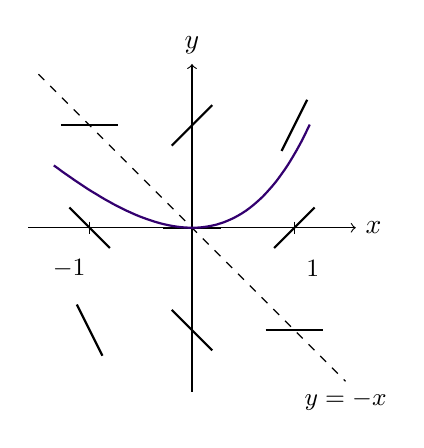
\begin{tikzpicture}[scale=1.3]
\draw[->] (-1.6,0) -- (1.6,0) node[right] {$x$};
\draw[->] (0,-1.6) -- (0,1.6) node[above] {$y$};
\draw[dashed] (-1.5,1.5) -- (1.5,-1.5) node[below] {\small $y=-x$};
\draw[thick] (-1.125,-0.750) -- (-0.875,-1.250);
\draw[thick] (-1.198,0.198) -- (-0.802,-0.198);
\draw[thick] (-1.280,1.000) -- (-0.720,1.000);
\draw[thick] (-0.198,-0.802) -- (0.198,-1.198);
\draw[thick] (-0.280,0.000) -- (0.280,0.000);
\draw[thick] (-0.198,0.802) -- (0.198,1.198);
\draw[thick] (0.720,-1.000) -- (1.280,-1.000);
\draw[thick] (0.802,-0.198) -- (1.198,0.198);
\draw[thick] (0.875,0.750) -- (1.125,1.250);
\draw[purple, thick] (-1.350,0.609) -- (-1.308,0.579) -- (-1.267,0.548) -- (-1.225,0.519) -- (-1.183,0.490) -- (-1.142,0.461) -- (-1.100,0.433) -- (-1.058,0.405) -- (-1.017,0.378) -- (-0.975,0.352) -- (-0.933,0.327) -- (-0.892,0.302) -- (-0.850,0.277) -- (-0.808,0.254) -- (-0.767,0.231) -- (-0.725,0.209) -- (-0.683,0.188) -- (-0.642,0.168) -- (-0.600,0.149) -- (-0.558,0.130) -- (-0.517,0.113) -- (-0.475,0.097) -- (-0.433,0.082) -- (-0.392,0.068) -- (-0.350,0.055) -- (-0.308,0.043) -- (-0.267,0.033) -- (-0.225,0.024) -- (-0.183,0.016) -- (-0.142,0.010) -- (-0.100,0.005) -- (-0.058,0.002) -- (-0.017,0.000) -- (0.025,0.000) -- (0.067,0.002) -- (0.108,0.006) -- (0.150,0.012) -- (0.192,0.020) -- (0.233,0.029) -- (0.275,0.042) -- (0.317,0.056) -- (0.358,0.073) -- (0.400,0.092) -- (0.442,0.114) -- (0.483,0.138) -- (0.525,0.165) -- (0.567,0.196) -- (0.608,0.229) -- (0.650,0.266) -- (0.692,0.305) -- (0.733,0.349) -- (0.775,0.396) -- (0.817,0.446) -- (0.858,0.501) -- (0.900,0.560) -- (0.942,0.623) -- (0.983,0.690) -- (1.025,0.762) -- (1.067,0.839) -- (1.108,0.921) -- (1.150,1.008);
\draw (1,0.06) -- (1,-0.06); \draw (-1,0.06) -- (-1,-0.06);
\node at (1.18,-0.4) {\small $1$};
\node at (-1.2,-0.4) {\small $-1$};
\end{tikzpicture}
\end{center}
\end{solution}

\item[(c)] Find the equilibrium solutions of $y'=y^2-4$ and decide whether nearby solutions move toward or away from each.
\begin{solution}
Equilibria are constant solutions, where $y'=0$: $y=2$ and $y=-2$. The sign of $y'=(y-2)(y+2)$ is positive for $y>2$, negative for $-2<y<2$, and positive for $y<-2$. Near $y=-2$, solutions above it decrease and solutions below it increase, so they move toward $y=-2$. Near $y=2$, solutions above increase and solutions below decrease, so they move away from $y=2$.
\end{solution}

\item[(d)] Euler's method with $h=0.5$ for $y'=x+y$, $y(0)=1$, to approximate $y(1)$. Over or under estimate?
\begin{solution}
Euler's method steps along the tangent line: $y_{k+1}=y_k+h\,F(x_k,y_k)$ with $F(x,y)=x+y$.
\[ y_1=1+0.5(0+1)=1.5, \qquad y_2=1.5+0.5(0.5+1.5)=2.5. \]
So $y(1)\approx2.5$. Differentiating the equation, $y''=1+y'=1+x+y>0$ along the solution here, so the solution is concave up and lies above its tangent lines. Euler's method underestimates. (The exact value is $2e-2\approx3.44$.)
\end{solution}

\item[(e)] Euler's method with $h=-1$ for $y'=y-x$, $y(1)=3$, to approximate $y(-1)$.
\begin{solution}
$y_{k+1}=y_k+h\,(y_k-x_k)$ with $h=-1$.
\[ y(0)\approx3+(-1)(3-1)=1, \qquad y(-1)\approx1+(-1)(1-0)=0. \]
\end{solution}

\item[(f)] Solve $\frac{dy}{dx}=xy^2$, $y(0)=1$. On what interval is the solution defined?
\begin{solution}
Separate: $y^{-2}\,dy=x\,dx$, so $-\frac1y=\frac{x^2}{2}+C$. At $x=0$, $-1=C$. Then $\frac1y=1-\frac{x^2}{2}$, so
\[ y=\frac{2}{2-x^2}. \]
This blows up where $x^2=2$. The interval containing $x=0$ on which it is defined is $(-\sqrt2,\sqrt2)$.
\end{solution}

\item[(g)] Solve $\frac{dy}{dx}=e^{x-y}$, $y(0)=\ln2$.
\begin{solution}
$e^{x-y}=e^xe^{-y}$, so separate: $e^y\,dy=e^x\,dx$ and $e^y=e^x+C$. At $x=0$, $2=1+C$, so $C=1$ and
\[ y=\ln(e^x+1). \]
\end{solution}

\item[(h)] Solve $\frac{dy}{dt}=3y-6$, $y(0)=5$.
\begin{solution}
$\frac{dy}{dt}=3(y-2)$. Separate: $\frac{dy}{y-2}=3\,dt$, so $\ln|y-2|=3t+C$ and $y-2=Ae^{3t}$ for a constant $A$. At $t=0$, $A=3$.
\[ y=2+3e^{3t}. \]
\end{solution}

\item[(i)] Bacteria grow at a rate proportional to size, from $200$ cells to $600$ in $2$ hours. Find $P(t)$ and when $P=5400$.
\begin{solution}
$\frac{dP}{dt}=kP$ gives $P(t)=200e^{kt}$. From $600=200e^{2k}$, $e^{2k}=3$, so $k=\frac{\ln3}{2}$ and
\[ P(t)=200\cdot3^{t/2}. \]
$5400=200\cdot3^{t/2}$ means $3^{t/2}=27=3^3$, so $t=6$ hours.
\end{solution}

\item[(j)] Logistic: $\frac{dP}{dt}=0.5P\left(1-\frac{P}{1000}\right)$, $P(0)=200$. Carrying capacity, equilibria, growth, and $P(t)$.
\begin{solution}
(i) The carrying capacity is $M=1000$. The equilibria are $P=0$ and $P=1000$.

(ii) For $0<P<1000$ both factors are positive, so $P$ increases. The rate $0.5P-\frac{0.5P^2}{1000}$ is a downward parabola in $P$ with roots $0$ and $1000$, so it is largest at the vertex $P=500$.

(iii) Separate with partial fractions: $\frac{1000}{P(1000-P)}=\frac1P+\frac{1}{1000-P}$, so $\ln\left|\frac{P}{1000-P}\right|=0.5t+C$ and $\frac{P}{1000-P}=Be^{0.5t}$ for a constant $B$. At $t=0$, $B=\frac{200}{800}=\frac14$. Solving for $P$,
\[ P(t)=\frac{1000}{1+4e^{-0.5t}}. \]
$P=500$ when $4e^{-0.5t}=1$, that is $t=2\ln4=4\ln2$.
\end{solution}

\end{enumerate}

\end{enumerate}

\end{document}
